\section{常系数方程}
\label{sec:lde-constant}

一个未知函数不够用时，状态就成了向量。设$\bm{A}\in\mathbb{R}^{n\times n}$是常数矩阵，考虑
\begin{equation}
 \dot{\bm{x}}(t)=\bm{A}\bm{x}(t),\qquad \bm{x}(t_0)=\bm{x}_0.
 \label{eq:lde-constant-system}
\end{equation}
标量情形的解是$\mathrm{e}^{(t-t_0)a}x_0$。向量情形需要回答：矩阵的“指数”是什么，它为什么能解方程，又怎样算出来？高阶标量方程随后会放进同一框架。

\subsection{矩阵指数解}
\label{sec:lde-matrix-exponential}

指数函数的幂级数只用到加法、数乘和乘幂，这些运算对方阵都有定义。于是把级数中的数$a$换成矩阵$\bm{A}$。

\begin{definition}[矩阵指数]
\label{def:lde-matrix-exponential}
对$\bm{A}\in\mathbb{R}^{n\times n}$和$t\in\mathbb{R}$，定义\term{矩阵指数}（matrix exponential）
\begin{equation}
 \mathrm{e}^{t\bm{A}}=\sum_{k=0}^{\infty}\frac{t^k\bm{A}^k}{k!}=\bm{I}+t\bm{A}+\frac{t^2\bm{A}^2}{2}+\cdots.
 \label{eq:lde-matrix-exponential}
\end{equation}
\end{definition}

下面的性质逐条对应标量指数的性质，只有第4条多了一个可交换的条件。

\begin{theorem}[矩阵指数的基本性质]
\label{thm:lde-matexp-properties}
设$\bm{A},\bm{B}\in\mathbb{R}^{n\times n}$，$s,t\in\mathbb{R}$。
\begin{enumerate}
 \item 级数~\eqref{eq:lde-matrix-exponential}绝对收敛，在$t$的有界集上一致收敛，并且
 \begin{equation}
  \lVert\mathrm{e}^{t\bm{A}}\rVert_2\leq\mathrm{e}^{\lvert t\rvert\lVert\bm{A}\rVert_2}.
  \label{eq:lde-matexp-bound}
 \end{equation}
 \item $\mathrm{e}^{0\bm{A}}=\bm{I}$，并且
 \begin{equation}
  \frac{\mathrm{d}}{\mathrm{d}t}\mathrm{e}^{t\bm{A}}=\bm{A}\mathrm{e}^{t\bm{A}}=\mathrm{e}^{t\bm{A}}\bm{A}.
  \label{eq:lde-matexp-derivative}
 \end{equation}
 \item 指数律成立，特别地，$\mathrm{e}^{t\bm{A}}$可逆，逆矩阵是$\mathrm{e}^{-t\bm{A}}$：
 \begin{equation}
  \mathrm{e}^{(t+s)\bm{A}}=\mathrm{e}^{t\bm{A}}\mathrm{e}^{s\bm{A}}.
  \label{eq:lde-matexp-group}
 \end{equation}
 \item 若$\bm{A}\bm{B}=\bm{B}\bm{A}$，则
 \begin{equation}
  \mathrm{e}^{t(\bm{A}+\bm{B})}=\mathrm{e}^{t\bm{A}}\mathrm{e}^{t\bm{B}}.
  \label{eq:lde-matexp-commuting}
 \end{equation}
 \item 若$\bm{V}$可逆，则
 \begin{equation}
  \mathrm{e}^{t\bm{V}\bm{B}\bm{V}^{-1}}=\bm{V}\mathrm{e}^{t\bm{B}}\bm{V}^{-1}.
  \label{eq:lde-matexp-similarity}
 \end{equation}
\end{enumerate}
\end{theorem}

\begin{proof}
(1)谱范数满足$\lVert\bm{A}^k\rVert_2\leq\lVert\bm{A}\rVert_2^k$，所以第$k$项的范数不超过$(\lvert t\rvert\lVert\bm{A}\rVert_2)^k/k!$。当$\lvert t\rvert\leq T$时，它被收敛的数值级数$\sum_k(T\lVert\bm{A}\rVert_2)^k/k!$的通项控制，一致收敛由优级数判别法得到。对这个不等式求和就是所述范数界。

(2)$t=0$时只剩首项$\bm{I}$。逐项求导得到
\[
 \sum_{k\geq1}\frac{t^{k-1}\bm{A}^k}{(k-1)!}=\bm{A}\sum_{j\geq0}\frac{t^{j}\bm{A}^{j}}{j!}.
\]
由(1)，导数级数在有界集上一致收敛，所以逐项求导合法。矩阵$\bm{A}$可以提到左边，也可以提到右边，因为它与自身的乘幂可交换。

(3)固定$s$，定义
\[
 \bm{Y}(t)=\mathrm{e}^{-t\bm{A}}\mathrm{e}^{(t+s)\bm{A}}.
\]
由(2)，
\[
 \dot{\bm{Y}}(t)=-\mathrm{e}^{-t\bm{A}}\bm{A}\mathrm{e}^{(t+s)\bm{A}}+\mathrm{e}^{-t\bm{A}}\bm{A}\mathrm{e}^{(t+s)\bm{A}}=\bm{0}.
\]
所以$\bm{Y}(t)=\bm{Y}(0)=\mathrm{e}^{s\bm{A}}$。取$s=0$得$\mathrm{e}^{-t\bm{A}}\mathrm{e}^{t\bm{A}}=\bm{I}$，方阵的左逆即逆。再用这个逆乘$\bm{Y}(t)=\mathrm{e}^{s\bm{A}}$的两边，就得到加法公式。

(4)$\bm{B}$与$\bm{A}$的每个乘幂可交换，所以$\bm{B}$与$\mathrm{e}^{t\bm{A}}$可交换。定义
\[
 \bm{Y}(t)=\mathrm{e}^{-t(\bm{A}+\bm{B})}\mathrm{e}^{t\bm{A}}\mathrm{e}^{t\bm{B}}.
\]
乘积求导得三项：
\[
 \dot{\bm{Y}}=\mathrm{e}^{-t(\bm{A}+\bm{B})}\bigl(-(\bm{A}+\bm{B})\mathrm{e}^{t\bm{A}}+\bm{A}\mathrm{e}^{t\bm{A}}+\mathrm{e}^{t\bm{A}}\bm{B}\bigr)\mathrm{e}^{t\bm{B}}.
\]
括号内由交换关系等于零，$\bm{Y}(t)=\bm{Y}(0)=\bm{I}$。再用(3)的逆矩阵乘回去。

(5)乘幂满足下式，其中相邻的$\bm{V}^{-1}\bm{V}$都消去了：
\[
 (\bm{V}\bm{B}\bm{V}^{-1})^k=\bm{V}\bm{B}^k\bm{V}^{-1}.
\]
代入级数，提出$\bm{V}$和$\bm{V}^{-1}$。
\end{proof}

\begin{theorem}[常系数齐次系统的解]
\label{thm:lde-constant-solution}
对任意$\bm{x}_0\in\mathbb{R}^n$，初值问题~\eqref{eq:lde-constant-system}在$\mathbb{R}$上有唯一解，它是
\begin{equation}
 \bm{x}(t)=\mathrm{e}^{(t-t_0)\bm{A}}\bm{x}_0.
 \label{eq:lde-constant-solution}
\end{equation}
\end{theorem}

\begin{proof}
由定理~\ref{thm:lde-matexp-properties}的(2)，式~\eqref{eq:lde-constant-solution}满足方程，$t=t_0$时等于$\bm{x}_0$。

反过来设$\bm{x}$是任意一个解，令$\bm{z}(t)=\mathrm{e}^{-(t-t_0)\bm{A}}\bm{x}(t)$。求导得
\[
 \dot{\bm{z}}=\mathrm{e}^{-(t-t_0)\bm{A}}(-\bm{A}\bm{x}+\dot{\bm{x}})=\bm{0}.
\]
所以$\bm{z}(t)=\bm{z}(t_0)=\bm{x}_0$，再乘$\mathrm{e}^{(t-t_0)\bm{A}}$就得到式~\eqref{eq:lde-constant-solution}。
\end{proof}

这个证明与积分因子完全平行：$\mathrm{e}^{-(t-t_0)\bm{A}}$扮演积分因子的角色，它和$\bm{A}$可交换，所以能够抵消方程右端。第~\ref{sec:lde-time-varying}节会看到，时变系数之所以困难，正是因为这种交换关系消失了。

先用级数算一个例子。取
\[
 \bm{J}_0=\begin{bmatrix}0&1\\-1&0\end{bmatrix},
\]
方程是$\dot{x}_1=x_2$、$\dot{x}_2=-x_1$。计算$\bm{J}_0^2=-\bm{I}$，级数的偶次项和奇次项分别凑成余弦和正弦：
\[
 \mathrm{e}^{t\bm{J}_0}=(\cos t)\bm{I}+(\sin t)\bm{J}_0=\begin{bmatrix}\cos t&\sin t\\-\sin t&\cos t\end{bmatrix}.
\]
矩阵的指数在这里是顺时针旋转。图~\ref{fig:lde-matexp-series}(a)画出从$(1,0)^{\top}$出发的轨道和截断到第$K$项的部分和。$K$越大，部分和贴住单位圆的时间越长。

图(b)是固定时刻的截断误差。余项首项的大小约为$t^{K+1}/(K+1)!$，$K$小于$t$时这一项还在增大，超过$t$之后才因阶乘而迅速下降，所以$t$越大需要的项数越多。

\begin{BookInlineFigure}
  \centering
  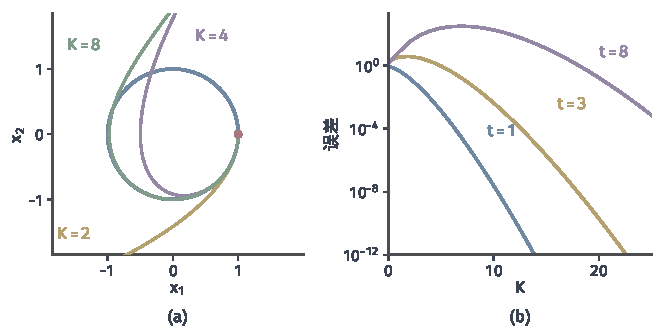
\includegraphics[width=112mm]{figures/06-differential-equations/01-ordinary-differential-equations/matplotlib/lde-matexp-series/figure.pdf}
  \caption{旋转矩阵$\bm{J}_0$的指数级数。(a)蓝色单位圆是精确轨道$\mathrm{e}^{t\bm{J}_0}(1,0)^{\top}$，彩色曲线是$t\in[0,1.5\pi]$上截断到第$K$项的部分和。(b)部分和与$\mathrm{e}^{t\bm{J}_0}$之差的谱范数，纵轴为对数，取$t=1,3,8$。}
  \label{fig:lde-matexp-series}
\end{BookInlineFigure}

\paragraph{对角化：解耦成独立的模式}
级数说明了矩阵指数是什么，计算时却要依靠矩阵的结构。若$\bm{A}$有$n$个线性无关的特征向量，就有$\bm{A}=\bm{V}\bm{\Lambda}\bm{V}^{-1}$，其中$\bm{V}$的列是特征向量$\bm{v}_i$，$\bm{\Lambda}$是特征值组成的对角阵。令$\bm{y}=\bm{V}^{-1}\bm{x}$，方程解耦成$n$个互不相干的标量方程：
\[
 \dot{y}_i=\lambda_iy_i,\qquad i=1,\ldots,n.
\]

记$\bm{w}_i^{\top}$为$\bm{V}^{-1}$的第$i$行。由定理~\ref{thm:lde-matexp-properties}的(5)和对角阵的指数，
\begin{equation}
 \mathrm{e}^{t\bm{A}}=\bm{V}\mathrm{e}^{t\bm{\Lambda}}\bm{V}^{-1}=\sum_{i=1}^{n}\mathrm{e}^{\lambda_it}\bm{v}_i\bm{w}_i^{\top}.
 \label{eq:lde-spectral-exponential}
\end{equation}
读法是：$\bm{w}_i^{\top}\bm{x}_0$量出初值在第$i$个特征方向上的分量，这个分量沿自己的方向按$\mathrm{e}^{\lambda_it}$变化。对角化以及下面用到的三角化（Schur形）的条件与计算，可参考\BookChapterRef{chap:eigen-spectral-decomposition}{卷二第6章“谱分解”}。

\begin{example}[贯穿全章的二维系统]
\label{ex:lde-running-system}
取
\[
 \bm{A}=\begin{bmatrix}0&1\\-2&-3\end{bmatrix}.
\]
特征多项式是$z^2+3z+2=(z+1)(z+2)$，特征值为$-1$和$-2$。解$(\bm{A}-\lambda\bm{I})\bm{v}=\bm{0}$，得到特征向量和它们组成的矩阵：
\[
 \bm{V}=\begin{bmatrix}1&1\\-1&-2\end{bmatrix},\qquad \bm{V}^{-1}=\begin{bmatrix}2&1\\-1&-1\end{bmatrix}.
\]
所以$\bm{w}_1^{\top}=(2,1)$，$\bm{w}_2^{\top}=(-1,-1)$。代入式~\eqref{eq:lde-spectral-exponential}，
\[
 \mathrm{e}^{t\bm{A}}=\mathrm{e}^{-t}\begin{bmatrix}2&1\\-2&-1\end{bmatrix}+\mathrm{e}^{-2t}\begin{bmatrix}-1&-1\\2&2\end{bmatrix}.
\]
取$t=0$，两个矩阵相加恰为$\bm{I}$，这是一次检验。取$\bm{x}_0=(1,0)^{\top}$，第一列给出
\[
 x_1(t)=2\mathrm{e}^{-t}-\mathrm{e}^{-2t},\qquad x_2(t)=-2\mathrm{e}^{-t}+2\mathrm{e}^{-2t}.
\]
再检验方程：$\dot{x}_1=-2\mathrm{e}^{-t}+2\mathrm{e}^{-2t}=x_2$，$\dot{x}_2=2\mathrm{e}^{-t}-4\mathrm{e}^{-2t}$，而
\[
 -2x_1-3x_2=2\mathrm{e}^{-t}-4\mathrm{e}^{-2t}.
\]
\end{example}

图~\ref{fig:lde-diagonal-modes}把同一批初值放在两个坐标系中。(a)的轨线弯曲，看不出规律；(b)用特征坐标后，两个坐标各自按$\mathrm{e}^{-t}$和$\mathrm{e}^{-2t}$收缩。$y_2$衰减得更快，所以轨线在到达原点前几乎都贴向$y_1$轴，在原坐标中表现为贴向$\bm{v}_1$方向。

\begin{BookInlineFigure}
  \centering
  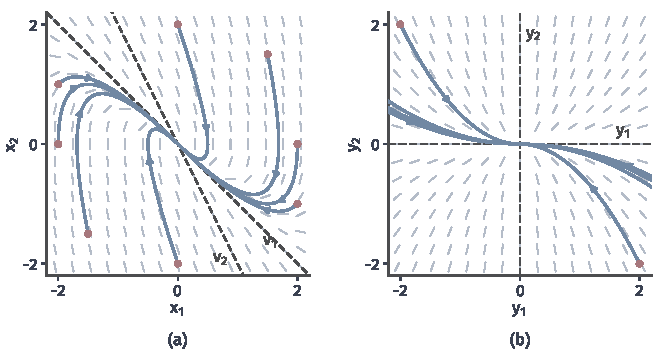
\includegraphics[width=112mm]{figures/06-differential-equations/01-ordinary-differential-equations/matplotlib/lde-diagonal-modes/figure.pdf}
  \caption{对角化解耦，系统取例~\ref{ex:lde-running-system}的$\bm{A}$。(a)原坐标的相平面，灰色短线是方向，蓝线是解，红点是初值，深灰虚线是特征方向$\bm{v}_1,\bm{v}_2$。(b)特征坐标$\bm{y}=\bm{V}^{-1}\bm{x}$中同一批解（超出显示范围的初值点未标出），特征方向成为坐标轴。}
  \label{fig:lde-diagonal-modes}
\end{BookInlineFigure}

\paragraph{复特征值：旋转与伸缩}
实矩阵可能有共轭复特征值$\alpha\pm\mathrm{i}\beta$（$\beta\neq0$）。式~\eqref{eq:lde-spectral-exponential}在复数域上仍然成立，但实系统的解是实的，更好的写法是看典型的二维块
\[
 \bm{A}=\begin{bmatrix}\alpha&\beta\\-\beta&\alpha\end{bmatrix}=\alpha\bm{I}+\beta\bm{J}_0.
\]
$\alpha\bm{I}$与任何矩阵可交换，由定理~\ref{thm:lde-matexp-properties}的(4)，
\begin{equation}
 \mathrm{e}^{t\bm{A}}=\mathrm{e}^{\alpha t}\begin{bmatrix}\cos\beta t&\sin\beta t\\-\sin\beta t&\cos\beta t\end{bmatrix}.
 \label{eq:lde-complex-block}
\end{equation}
实部$\alpha$负责伸缩，虚部$\beta$负责旋转的快慢。图~\ref{fig:lde-spiral}取$\alpha=-1$、$\beta=2$：相平面上是向内的螺线，分量则是被$\pm\mathrm{e}^{-t}$夹住的振荡。一般实矩阵的共轭特征值对，可以用实的相似变换化成这种二维块。

\begin{BookInlineFigure}
  \centering
  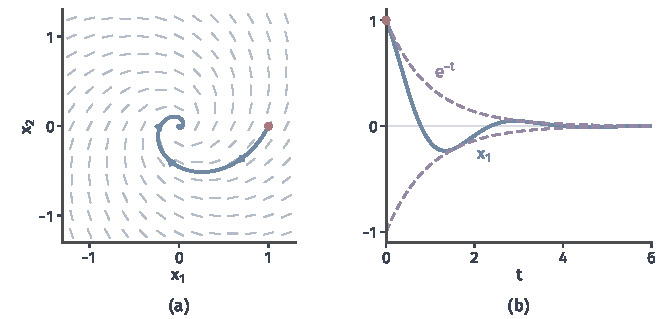
\includegraphics[width=112mm]{figures/06-differential-equations/01-ordinary-differential-equations/matplotlib/lde-spiral/figure.pdf}
  \caption{复特征值对应旋转与伸缩，$\bm{A}=\left[\begin{smallmatrix}-1&2\\-2&-1\end{smallmatrix}\right]$，特征值$-1\pm2\mathrm{i}$，初值$(1,0)^{\top}$（红点）。(a)相平面的螺线。(b)分量$x_1=\mathrm{e}^{-t}\cos2t$（蓝）与紫色虚线包络$\pm\mathrm{e}^{-t}$。}
  \label{fig:lde-spiral}
\end{BookInlineFigure}

\paragraph{三角形式：逐行回代}
不能对角化时，总可以退到三角形式。任意复方阵都酉相似于上三角阵$\bm{T}$，对角元是全部特征值；定理~\ref{thm:lde-matexp-properties}对复矩阵同样成立，证明不变。上三角系统的最后一行不含其他分量，可以先解出；倒数第二行以它为输入，又是一个一阶线性方程。于是第~\ref{sec:lde-first-order}节的公式可以逐行使用。

看一个具体的矩阵：
\[
 \bm{A}=\begin{bmatrix}-1&1\\0&-2\end{bmatrix}.
\]
第二行给出$x_2(t)=\mathrm{e}^{-2t}x_2(0)$。第一行是$\dot{x}_1=-x_1+x_2$，由式~\eqref{eq:lde-scalar-solution}，
\[
 x_1(t)=\mathrm{e}^{-t}x_1(0)+\Bigl(\int_0^t\mathrm{e}^{-(t-s)}\mathrm{e}^{-2s}\,\mathrm{d}s\Bigr)x_2(0).
\]
括号内的积分提出$\mathrm{e}^{-t}$后等于
\[
 \mathrm{e}^{-t}\int_0^t\mathrm{e}^{-s}\,\mathrm{d}s=\mathrm{e}^{-t}-\mathrm{e}^{-2t},
\]
所以
\[
 x_1(t)=\mathrm{e}^{-t}x_1(0)+(\mathrm{e}^{-t}-\mathrm{e}^{-2t})x_2(0).
\]

现在把第二个对角元也改成$-1$。积分变成$\int_0^t\mathrm{e}^{-(t-s)}\mathrm{e}^{-s}\,\mathrm{d}s$，被积函数恒等于$\mathrm{e}^{-t}$，与$s$无关，积分结果是$t\mathrm{e}^{-t}$。多项式因子就这样出现了：上一行的输出含有与下一行自身相同的模式，贡献按时间不断累积，而不是像前一例那样互相抵消。

\paragraph{Jordan块：不能只看特征值}
比较两个$2\times2$矩阵$-\bm{I}$和
\[
 \bm{J}=\begin{bmatrix}-1&1\\0&-1\end{bmatrix}.
\]
它们的特征多项式都是$(z+1)^2$，特征值完全相同，指数却不同。一般地，形如$\lambda\bm{I}+\bm{N}$的$s$阶矩阵称为Jordan块，其中$\bm{N}$的超对角元为$1$、其余元素为$0$，满足$\bm{N}^s=\bm{0}$。$\lambda\bm{I}$与$\bm{N}$可交换，由定理~\ref{thm:lde-matexp-properties}的(4)，级数在第$s$项截断：
\begin{equation}
 \mathrm{e}^{t(\lambda\bm{I}+\bm{N})}=\mathrm{e}^{\lambda t}\sum_{j=0}^{s-1}\frac{t^j\bm{N}^j}{j!}.
 \label{eq:lde-jordan-exponential}
\end{equation}

对上面的$\bm{J}$，$s=2$，结果是
\[
 \mathrm{e}^{t\bm{J}}=\mathrm{e}^{-t}\begin{bmatrix}1&t\\0&1\end{bmatrix},
\]
而$\mathrm{e}^{-t\bm{I}}=\mathrm{e}^{-t}\bm{I}$没有$t$项。二者的差别在于特征向量的个数。$-\bm{I}$的特征向量张成整个平面，$\bm{J}$只有$\bm{e}_1$一个方向。卷二讨论矩阵幂时已经遇到同样的现象，$\bm{J}^k$中出现了$k$的多项式因子，可参考\BookChapterRef{chap:linear-recurrence-stability}{卷二第10章“线性递推的收敛与稳定性”}。

缺少的方向由\term{广义特征向量}（generalized eigenvector）补上：满足$(\bm{A}-\lambda\bm{I})^2\bm{v}=\bm{0}$而$\bm{u}=(\bm{A}-\lambda\bm{I})\bm{v}\neq\bm{0}$的向量$\bm{v}$。此时$\bm{u}$是特征向量，并且从$\bm{v}$出发的解是
\begin{equation}
 \bm{x}(t)=\mathrm{e}^{\lambda t}\bigl(\bm{v}+t\bm{u}\bigr).
 \label{eq:lde-generalized-solution}
\end{equation}
对$\bm{J}$取$\bm{v}=\bm{e}_2$，则$\bm{u}=\bm{e}_1$，式~\eqref{eq:lde-generalized-solution}与$\mathrm{e}^{t\bm{J}}$的第二列一致。

图~\ref{fig:lde-jordan-vs-diagonal}把差别画了出来。(a)中每条轨线都是直线，(b)中轨线都沿唯一的特征方向进入原点，看起来像被拧过。图~\ref{fig:lde-jordan-chain}给出多项式因子的另一种读法：Jordan块是一串相同的一阶系统首尾相接，每经过一级，就多累积一次，多一个$t$的幂。

\begin{BookInlineFigure}
  \centering
  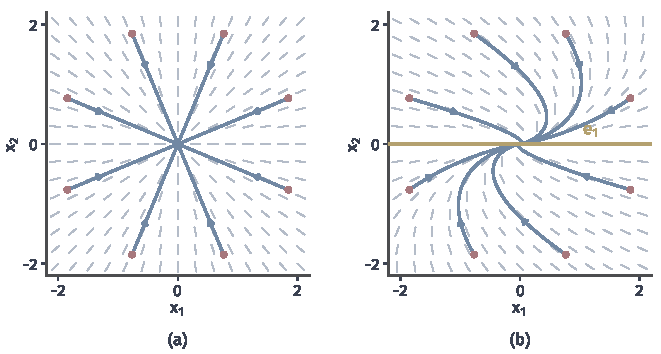
\includegraphics[width=112mm]{figures/06-differential-equations/01-ordinary-differential-equations/matplotlib/lde-jordan-vs-diagonal/figure.pdf}
  \caption{特征值相同而相图不同，红点是半径为$2$的圆上的初值。(a)$\bm{A}=-\bm{I}$，每个方向都是特征方向，轨线是直线。(b)$\bm{A}=\bm{J}$，只有黄色的$\bm{e}_1$轴是特征方向，其余轨线都沿它的方向进入原点。}
  \label{fig:lde-jordan-vs-diagonal}
\end{BookInlineFigure}

\begin{BookInlineFigure}
  \centering
  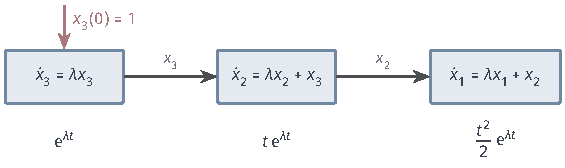
\includegraphics[width=96mm]{figures/06-differential-equations/01-ordinary-differential-equations/tikz/lde-jordan-chain/figure.pdf}
  \caption{三阶Jordan块看作一阶系统的串联。方框中是三个分量的方程，红色箭头表示只给$x_3$非零初值，方框下方是相应分量的响应。每一级的输入都含有该级自身的模式$\mathrm{e}^{\lambda t}$，于是响应多一次累积，得到$t$的更高次幂。}
  \label{fig:lde-jordan-chain}
\end{BookInlineFigure}

只看特征值还会错过有限时间内的放大。取
\[
 \bm{A}=\begin{bmatrix}-1&10\\0&-1\end{bmatrix},\qquad \bm{x}_0=\begin{bmatrix}0\\1\end{bmatrix}.
\]
把$\bm{N}$换成$10\bm{N}$，式~\eqref{eq:lde-jordan-exponential}给出
\[
 x_1(t)=10t\mathrm{e}^{-t},\qquad x_2(t)=\mathrm{e}^{-t}.
\]
两个特征值都是$-1$，看上去每个模式都在衰减，$x_1$却从$0$升到$t=1$处的$10/\mathrm{e}\approx3.68$，然后才下降，见图~\ref{fig:lde-jordan-transient}。放大来自对角线上方的耦合，特征值感受不到它。

\begin{BookInlineFigure}
  \centering
  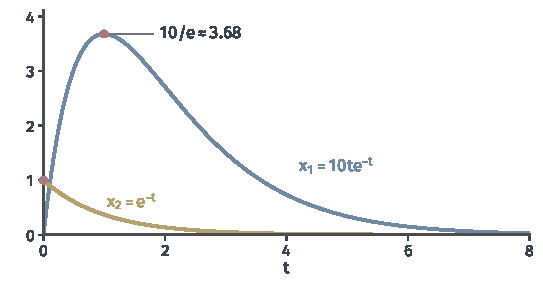
\includegraphics[width=92mm]{figures/06-differential-equations/01-ordinary-differential-equations/matplotlib/lde-jordan-transient/figure.pdf}
  \caption{重特征值带来的有限时间放大。$\bm{A}=\left[\begin{smallmatrix}-1&10\\0&-1\end{smallmatrix}\right]$，$\bm{x}_0=(0,1)^{\top}$。蓝线是$x_1$，在$t=1$达到峰值（右侧红点）；黄线是$x_2$，从左侧红点单调下降。}
  \label{fig:lde-jordan-transient}
\end{BookInlineFigure}

\paragraph{解的一般形状}
三角形式的回代可以写成一个对所有矩阵都成立的结论。

\begin{theorem}[矩阵指数的元素]
\label{thm:lde-exponential-shape}
设$\bm{A}\in\mathbb{R}^{n\times n}$的互异特征值为$\lambda_1,\ldots,\lambda_r$，代数重数为$m_1,\ldots,m_r$。则$\mathrm{e}^{t\bm{A}}$的每个元素都是下列函数的线性组合：
\begin{equation}
 t^j\mathrm{e}^{\lambda_it},\qquad 0\leq j<m_i,\quad i=1,\ldots,r.
 \label{eq:lde-exponential-shape}
\end{equation}
组合系数一般是复数。
\end{theorem}

\begin{proof}
由定理~\ref{thm:lde-matexp-properties}的(5)，只需证明上三角阵$\bm{T}$的情形。设$\bm{T}$的对角元为$\tau_1,\ldots,\tau_n$，解$\dot{\bm{x}}=\bm{T}\bm{x}$。从$i=n$往回归纳，证明$x_i$是若干$t^j\mathrm{e}^{\lambda t}$的组合，其中$\lambda\in\{\tau_i,\ldots,\tau_n\}$，$j$小于$\lambda$在$\tau_i,\ldots,\tau_n$中出现的次数。

$i=n$时$x_n=\mathrm{e}^{\tau_nt}x_n(0)$。设结论对$i+1,\ldots,n$成立。第$i$行是以$\sum_{k>i}T_{i,k}x_k$为输入的一阶线性方程，所以只要看一项输入$s^j\mathrm{e}^{\lambda s}$产生什么：
\[
 \int_0^t\mathrm{e}^{\tau_i(t-s)}s^j\mathrm{e}^{\lambda s}\,\mathrm{d}s=\mathrm{e}^{\tau_it}\int_0^ts^j\mathrm{e}^{(\lambda-\tau_i)s}\,\mathrm{d}s.
\]
若$\lambda\neq\tau_i$，分部积分$j$次得到次数至多为$j$的多项式乘$\mathrm{e}^{\lambda t}$，再加常数乘$\mathrm{e}^{\tau_it}$，幂次不升。若$\lambda=\tau_i$，积分等于$t^{j+1}/(j+1)$，幂次升一，而$\tau_i$在列表中恰好多出现一次。两种情形都保持归纳假设。
\end{proof}

定理说明指数、振荡和多项式因子是常系数线性系统仅有的三种成分：实部给出指数，虚部给出振荡，重根可能给出多项式。这里的“可能”不能省略，$-\bm{I}$就没有多项式因子。利用Jordan标准形可以把幂次上限收紧为“$j$小于$\lambda_i$的最大Jordan块阶数”，Jordan标准形的存在性证明较长，读者可查阅线性代数教材。

特征值的实部决定解在$t\to\infty$时的走向，但判断长期稳定还要考虑实部为零的特征值和Jordan块的大小，也要处理非线性系统，相关判据可参考\BookChapterRef{chap:dynamical-systems-long-term}{卷九第1章“动力系统与轨迹的长期行为”}。本章只关心解在有限时间上的形状。

\subsection{高阶标量方程}
\label{sec:lde-high-order}

质点在弹簧上的振动由二阶方程描述，电路和梁的问题还会出现更高阶的方程。记$\mathrm{D}=\mathrm{d}/\mathrm{d}t$，常系数$n$阶线性方程写作
\begin{equation}
 \mathrm{D}^nx+a_{n-1}\mathrm{D}^{n-1}x+\cdots+a_1\mathrm{D}x+a_0x=g(t),
 \label{eq:lde-high-order}
\end{equation}
其中系数$a_0,\ldots,a_{n-1}$是实常数。初值要给齐$x,\mathrm{D}x,\ldots,\mathrm{D}^{n-1}x$在$t_0$的值，共$n$个数。多项式$p(z)=z^n+a_{n-1}z^{n-1}+\cdots+a_0$称为方程的特征多项式，于是方程可以简写成$p(\mathrm{D})x=g$。

\paragraph{状态降阶}
第~\ref{chap:ordinary-differential-equations}章用位移和速度描述摆的状态，高阶方程也一样。令$x_k=\mathrm{D}^{k-1}x$（$k=1,\ldots,n$），前$n-1$个分量的方程就是定义$\dot{x}_k=x_{k+1}$，最后一个分量由方程~\eqref{eq:lde-high-order}解出。写成矩阵形式：
\begin{equation}
 \dot{\bm{x}}=\bm{C}\bm{x}+g(t)\bm{e}_n,\qquad
 \bm{C}=\begin{bmatrix}0&1&&\\&\ddots&\ddots&\\&&0&1\\-a_0&-a_1&\cdots&-a_{n-1}\end{bmatrix}.
 \label{eq:lde-companion}
\end{equation}
$\bm{C}$称为\term{友矩阵}（companion matrix）。例~\ref{ex:lde-running-system}的矩阵正是$p(z)=z^2+3z+2$的友矩阵。

图~\ref{fig:lde-companion-chain}把$n=3$的情形画成积分器串联。每个积分器保存一个状态分量，也就是系统需要“记住”的一个量，这也解释了为什么要给$n$个初值。

\begin{BookInlineFigure}
  \centering
  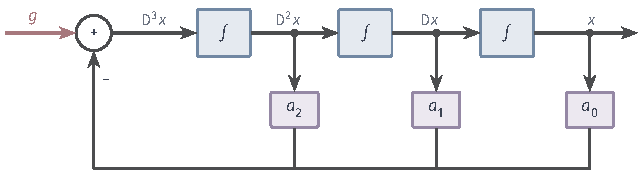
\includegraphics[width=108mm]{figures/06-differential-equations/01-ordinary-differential-equations/tikz/lde-companion-chain/figure.pdf}
  \caption{三阶方程$\mathrm{D}^3x+a_2\mathrm{D}^2x+a_1\mathrm{D}x+a_0x=g$的状态结构。蓝框是积分器，输出依次为状态分量$\mathrm{D}^2x,\mathrm{D}x,x$；紫框是系数，反馈后与红色输入$g$在求和点相减，得到最高阶导数。}
  \label{fig:lde-companion-chain}
\end{BookInlineFigure}

\begin{lemma}[友矩阵的谱]
\label{lem:lde-companion}
$\bm{C}$的特征多项式是$p$。对$\bm{C}$的每个特征值$\lambda$，特征子空间都是一维的，由下面的向量张成：
\begin{equation}
 \bm{v}(\lambda)=(1,\lambda,\lambda^2,\ldots,\lambda^{n-1})^{\top}.
 \label{eq:lde-companion-eigenvector}
\end{equation}
\end{lemma}

\begin{proof}
把$z\bm{I}-\bm{C}$的第$k$列乘$z^{k-1}$加到第$1$列（$k=2,\ldots,n$），行列式不变。逐行计算，新的第$1$列是$(0,\ldots,0,p(z))^{\top}$。

沿第$1$列展开，代数余子式对应的$n-1$阶子矩阵是下三角阵，对角元全为$-1$，行列式为$(-1)^{n-1}$。它再乘符号$(-1)^{n+1}$，结果是
\[
 \det(z\bm{I}-\bm{C})=(-1)^{n+1}(-1)^{n-1}p(z)=p(z).
\]

设$\bm{C}\bm{v}=\lambda\bm{v}$。前$n-1$行给出$v_{k+1}=\lambda v_k$，所以$\bm{v}$由$v_1$决定，并且$\bm{v}=v_1\bm{v}(\lambda)$。这就是特征子空间的一维性。
\end{proof}

引理的第二部分有直接的后果：若$\lambda$是$p$的$m$重根，$\bm{C}$在$\lambda$上只有一个Jordan块，阶数就是$m$。所以高阶标量方程不可能出现$-\bm{I}$那样“重特征值却没有多项式因子”的情况，重根一定带来$t,\ldots,t^{m-1}$。

\paragraph{基本解的列表}
上面的结论也可以直接从算子分解得到。常系数算子彼此可交换，$p(\mathrm{D})$可按根分解。关键的计算只有一步：
\[
 (\mathrm{D}-\lambda)\bigl(t^j\mathrm{e}^{\lambda t}\bigr)=jt^{j-1}\mathrm{e}^{\lambda t}.
\]
每作用一次$\mathrm{D}-\lambda$，$t$的幂次降一，所以$(\mathrm{D}-\lambda)^m$把$t^j\mathrm{e}^{\lambda t}$（$j<m$）变成零。

\begin{theorem}[高阶齐次方程的基本解]
\label{thm:lde-high-order-basis}
设$p(z)=\prod_{i=1}^{r}(z-\lambda_i)^{m_i}$，$\lambda_i$互异，$\sum_im_i=n$。则方程$p(\mathrm{D})x=0$的复值解构成$n$维线性空间，下列$n$个函数是它的一组基：
\begin{equation}
 t^j\mathrm{e}^{\lambda_it},\qquad 0\leq j<m_i,\quad i=1,\ldots,r.
 \label{eq:lde-high-order-basis}
\end{equation}
系数为实数时，一对共轭根$\alpha\pm\mathrm{i}\beta$对应的函数可以换成实函数$t^j\mathrm{e}^{\alpha t}\cos\beta t$和$t^j\mathrm{e}^{\alpha t}\sin\beta t$。
\end{theorem}

\begin{proof}
由上面的计算，这$n$个函数都是解。解空间的维数是$n$：由定理~\ref{thm:lde-constant-solution}，把解对应到初始状态$(x(0),\ldots,\mathrm{D}^{n-1}x(0))$是线性双射。

只需证明线性无关。假设存在非平凡关系$\sum_{i=1}^{r}q_i(t)\mathrm{e}^{\lambda_it}=0$，其中多项式$q_i$都不为零，$\lambda_i$互异，并取其中$r$最小的一个。$r=1$时$q_1\equiv0$，矛盾。

设$r\geq2$。乘$\mathrm{e}^{-\lambda_rt}$，再求导$\deg q_r+1$次，把$q_r$消去。其余每一项形如$q\mathrm{e}^{\mu t}$，$\mu=\lambda_i-\lambda_r\neq0$，而
\[
 \mathrm{D}(q\mathrm{e}^{\mu t})=(\dot{q}+\mu q)\mathrm{e}^{\mu t}.
\]
多项式的次数不变，首项系数乘$\mu$。所以得到一个只有$r-1$个指数的非平凡关系，与$r$的最小性矛盾。

系数为实数时，共轭根成对出现且重数相同。$t^j\mathrm{e}^{\alpha t}\cos\beta t$和$t^j\mathrm{e}^{\alpha t}\sin\beta t$分别是$t^j\mathrm{e}^{(\alpha\pm\mathrm{i}\beta)t}$的半和与半差（后者再除以$\mathrm{i}$），两组函数张成同一个空间。
\end{proof}

\paragraph{二阶振动方程}
质点受弹簧恢复力和阻尼时，满足$\ddot{x}+b\dot{x}+cx=0$，其中$b,c$是正常数。特征方程$z^2+bz+c=0$的判别式把运动分成三类。下面三个例子都取$x(0)=1$、$\dot{x}(0)=0$，只改变根的形状。

实根$p(z)=z^2+3z+2$，根为$-1,-2$。设$x=C_1\mathrm{e}^{-t}+C_2\mathrm{e}^{-2t}$，初值给出$C_1+C_2=1$和$-C_1-2C_2=0$，于是
\[
 x(t)=2\mathrm{e}^{-t}-\mathrm{e}^{-2t}.
\]

重根$p(z)=z^2+2z+1$，根为$-1$（二重）。设$x=(C_1+C_2t)\mathrm{e}^{-t}$，初值给出$C_1=1$和$-C_1+C_2=0$，于是
\[
 x(t)=(1+t)\mathrm{e}^{-t}.
\]

复根$p(z)=z^2+2z+5$，根为$-1\pm2\mathrm{i}$。设$x=\mathrm{e}^{-t}(C_1\cos2t+C_2\sin2t)$，初值给出$C_1=1$和$-C_1+2C_2=0$，于是
\[
 x(t)=\mathrm{e}^{-t}\Bigl(\cos2t+\frac12\sin2t\Bigr).
\]

图~\ref{fig:lde-damped-cases}比较这三条曲线。实根时质点单调回到平衡位置，复根时越过平衡位置来回摆动。重根恰好是两种情形的分界，它没有越过平衡位置，多项式因子$1+t$让它在开始阶段下降得比实根情形慢。三种情形及其物理名称见表~\ref{tab:lde-second-order}。

\begin{BookInlineFigure}
  \centering
  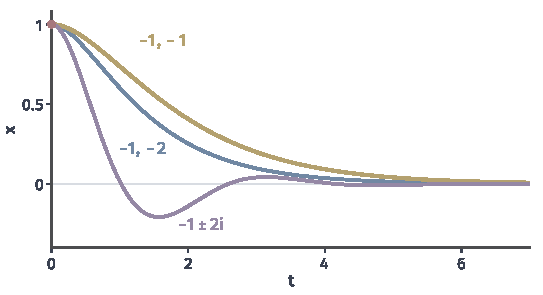
\includegraphics[width=92mm]{figures/06-differential-equations/01-ordinary-differential-equations/matplotlib/lde-damped-cases/figure.pdf}
  \caption{同一初值$x(0)=1$、$\dot{x}(0)=0$（红点）下的三类二阶方程，线旁标注特征根。蓝线：实根$-1,-2$。黄线：重根$-1,-1$。紫线：复根$-1\pm2\mathrm{i}$。}
  \label{fig:lde-damped-cases}
\end{BookInlineFigure}

\begin{BookInlineTable}
  \centering
  \caption{二阶常系数齐次方程的三类根。}
  \label{tab:lde-second-order}
  \begin{tabular}{lll}
    \toprule
    根的形状 & 基本解 & 运动形式\\
    \midrule
    相异实根$\lambda_1,\lambda_2$ & $\mathrm{e}^{\lambda_1t},\ \mathrm{e}^{\lambda_2t}$ & 过阻尼：不振荡\\
    二重根$\lambda$ & $\mathrm{e}^{\lambda t},\ t\mathrm{e}^{\lambda t}$ & 临界阻尼：不振荡的边界\\
    共轭复根$\alpha\pm\mathrm{i}\beta$ & $\mathrm{e}^{\alpha t}\cos\beta t,\ \mathrm{e}^{\alpha t}\sin\beta t$ & 欠阻尼：衰减振荡\\
    \bottomrule
  \end{tabular}
\end{BookInlineTable}

\paragraph{重根是两个根相撞}
重根的$t\mathrm{e}^{\lambda t}$看上去来得突然，用连续变化的系数看却很自然。考虑$\ddot{x}+2c\dot{x}+x=0$，根为$-c\pm\sqrt{c^2-1}$。图~\ref{fig:lde-root-locus}(a)显示，$c$从$0$增大到$1$时，一对共轭根沿单位圆向左靠拢，在$c=1$相撞于$-1$，然后沿实轴分开。

相撞时两个基本解变成同一个函数，线性无关性似乎丢失了。补救办法是取差商。令两根为$-1$和$-1-\varepsilon$，它们的基本解之差除以$\varepsilon$仍是解，而
\[
 \lim_{\varepsilon\to0}\frac{\mathrm{e}^{-t}-\mathrm{e}^{-(1+\varepsilon)t}}{\varepsilon}=t\mathrm{e}^{-t}.
\]
这个极限就是$\mathrm{e}^{\lambda t}$对$\lambda$的导数。图(b)中$\varepsilon$减小时差商曲线逐步靠近$t\mathrm{e}^{-t}$。两个靠得很近的根已经几乎产生了线性增长的因子，重根只是这个过程的极限。

\begin{BookInlineFigure}
  \centering
  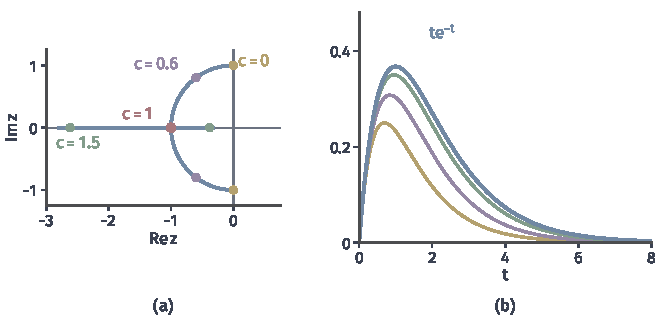
\includegraphics[width=112mm]{figures/06-differential-equations/01-ordinary-differential-equations/matplotlib/lde-root-locus/figure.pdf}
  \caption{根的相撞与多项式因子。(a)$z^2+2cz+1$的根随$c$的移动：$c=0$时在虚轴，$c=0.6$时在单位圆上，$c=1$时相撞于红点，$c=1.5$时分开在实轴上。(b)根为$-1,-1-\varepsilon$时的差商$(\mathrm{e}^{-t}-\mathrm{e}^{-(1+\varepsilon)t})/\varepsilon$，黄、紫、绿线依次取$\varepsilon=1,0.4,0.1$，蓝线是极限$t\mathrm{e}^{-t}$。}
  \label{fig:lde-root-locus}
\end{BookInlineFigure}
